\documentclass[12pt]{article}
\usepackage{amsmath, amssymb}
\usepackage{geometry}
\usepackage{graphicx}
\usepackage{hyperref}
\geometry{margin=1in}

\title{A Cyclic 4D-Time Universe Model: Bounce, Expansion, and Turnaround Controlled by Closed Time Geometry}
\author{Jacob L. Powell}
\date{\today}

\begin{document}
\maketitle

\begin{abstract}
We propose a conceptual cosmological framework in which the fourth dimension---time---is 
not infinite, but cyclic and bounded. This closed time geometry provides a natural mechanism 
for both the initiation of cosmic expansion (the bounce) and its termination (the turnaround), 
removing the need for external triggers. We derive an effective Friedmann equation, inspired by 
Loop Quantum Cosmology (LQC) \cite{Ashtekar2006,Bojowald2001}, that incorporates quantum 
corrections to avoid singularities, and show how a large-$a$ turnaround can arise through curvature 
or an effective negative cosmological term. The bounce is interpreted as a single-frame quantum 
state, linking emergent time concepts \cite{Hartle1983,Rovelli2017} with cyclic and conformal 
cosmological models \cite{Steinhardt2002,Penrose2010}.
\end{abstract}

\section{Introduction}
The classical theory of general relativity predicts singularities at the Big Bang and inside 
black holes, where the equations cease to be valid. Loop Quantum Cosmology (LQC) provides 
a resolution through quantum corrections that replace singularities with bounces 
\cite{Ashtekar2006,Bojowald2001}. Other cyclic approaches, such as the ekpyrotic/cyclic 
scenario \cite{Steinhardt2002}, posit a sequence of universes but often leave the termination 
of expansion unspecified. Penrose's Conformal Cyclic Cosmology (CCC) \cite{Penrose2010} 
offers an alternative by identifying the remote future of one aeon with the Big Bang of the 
next through conformal rescaling. 

The proposal developed here differs in a key way: time itself is treated as a closed arc, 
with expansion and contraction bounded by its periodicity. This \emph{cyclic 4D-time} ansatz 
eliminates the need for ad hoc triggers and provides a unified geometric controller for both 
the bounce and the turnaround.

\section{Framework}
\subsection{Cyclic Time Ansatz (Derived Periodicity)}
We posit periodic cosmic time $\tau \in [0,T)$ such that $a(\tau+T)=a(\tau)$. Turning points
occur at $a_{\min}$ (bounce) and $a_{\max}$ (turnaround), where $\dot a=0$.
From the effective Friedmann equation (Sec.~\ref{sec:effFriedmann}),
\begin{equation}
\dot a^2 = a^2\Bigg[\frac{8\pi G}{3}\rho(a)\left(1-\frac{\rho(a)}{\rho_c}\right)+\frac{\Lambda}{3}-\frac{k}{a^2}\Bigg]
\equiv -V_{\rm eff}(a).
\end{equation}
The cycle period is then
\begin{equation}
T = 2\int_{a_{\min}}^{a_{\max}}\frac{da}{\sqrt{-V_{\rm eff}(a)}},
\end{equation}
which is finite if both turning points exist. A convenient illustrative ansatz is
\begin{equation}
a(\tau) = a_{\min}+(a_{\max}-a_{\min})\sin^2\!\Big(\frac{\pi \tau}{T}\Big).
\end{equation}

\subsection{Effective Friedmann Equation from a Hamiltonian}
\label{sec:effFriedmann}
Following LQC, the effective Hamiltonian constraint is
\begin{equation}
\mathcal{C}_{\rm eff}=-\frac{3}{8\pi G\gamma^2\lambda^2}a\sin^2(\lambda b)+\rho(a)a^3=0,
\end{equation}
with Barbero--Immirzi parameter $\gamma$ and area gap $\lambda=\sqrt{\Delta}$.
This yields the modified Friedmann equation
\begin{equation}
H^2=\frac{8\pi G}{3}\rho(a)\left(1-\frac{\rho(a)}{\rho_c}\right)+\frac{\Lambda}{3}-\frac{k}{a^2},
\quad \rho_c=\frac{3}{8\pi G\gamma^2\lambda^2}.
\end{equation}
For $\rho(a)=\rho_{r0}a^{-4}+\rho_{m0}a^{-3}+\rho_\Lambda$:

\paragraph{Bounce condition.} At $a=a_{\min}$, $H=0$ gives $\rho=\rho_c$ and $\ddot a>0$, 
so the turning point is a stable minimum.

\paragraph{Turnaround condition.} At $a=a_{\max}$, $H=0$ implies
\begin{equation}
\frac{8\pi G}{3}\rho(a_{\max})\left(1-\frac{\rho(a_{\max})}{\rho_c}\right)+\frac{\Lambda}{3}-\frac{k}{a_{\max}^2}=0,
\end{equation}
linking $a_{\max}$ to observable parameters $(\Omega_{m0},\Omega_{r0},\Omega_{\Lambda0},\Omega_{k0})$.

\section{Results (Toy Examples)}
\subsection{Cyclic Scale Factor}
Figure~\ref{fig:atau} shows an illustrative periodic $a(\tau)$ with bounce and turnaround.

\begin{figure}[h]
\centering
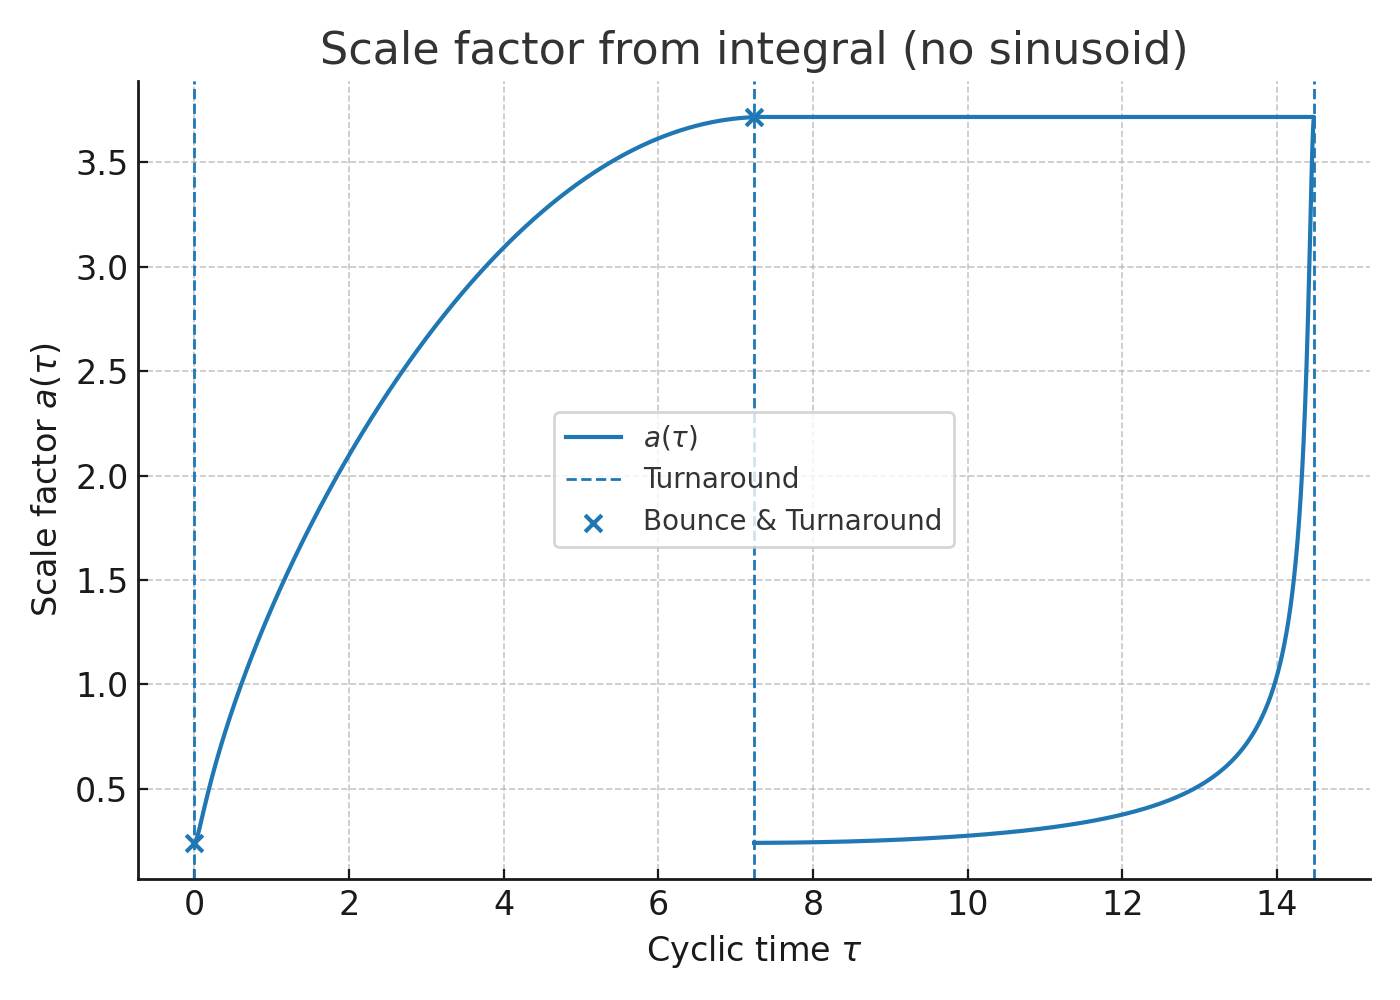
\includegraphics[width=0.7\linewidth]{figures/plot_a_tau_from_integral.png}
\caption{Cyclic time ansatz: $a(\tau)$ with bounce ($\tau=0$) and turnaround ($\tau=T/2$).}
\label{fig:atau}
\end{figure}

\subsection{Effective $H^2(a)$ with Two Turning Points}
Figure~\ref{fig:h2a} shows a toy $H^2(a)$ with both a small-$a$ bounce and a large-$a$ turnaround.

\begin{figure}[h]
\centering
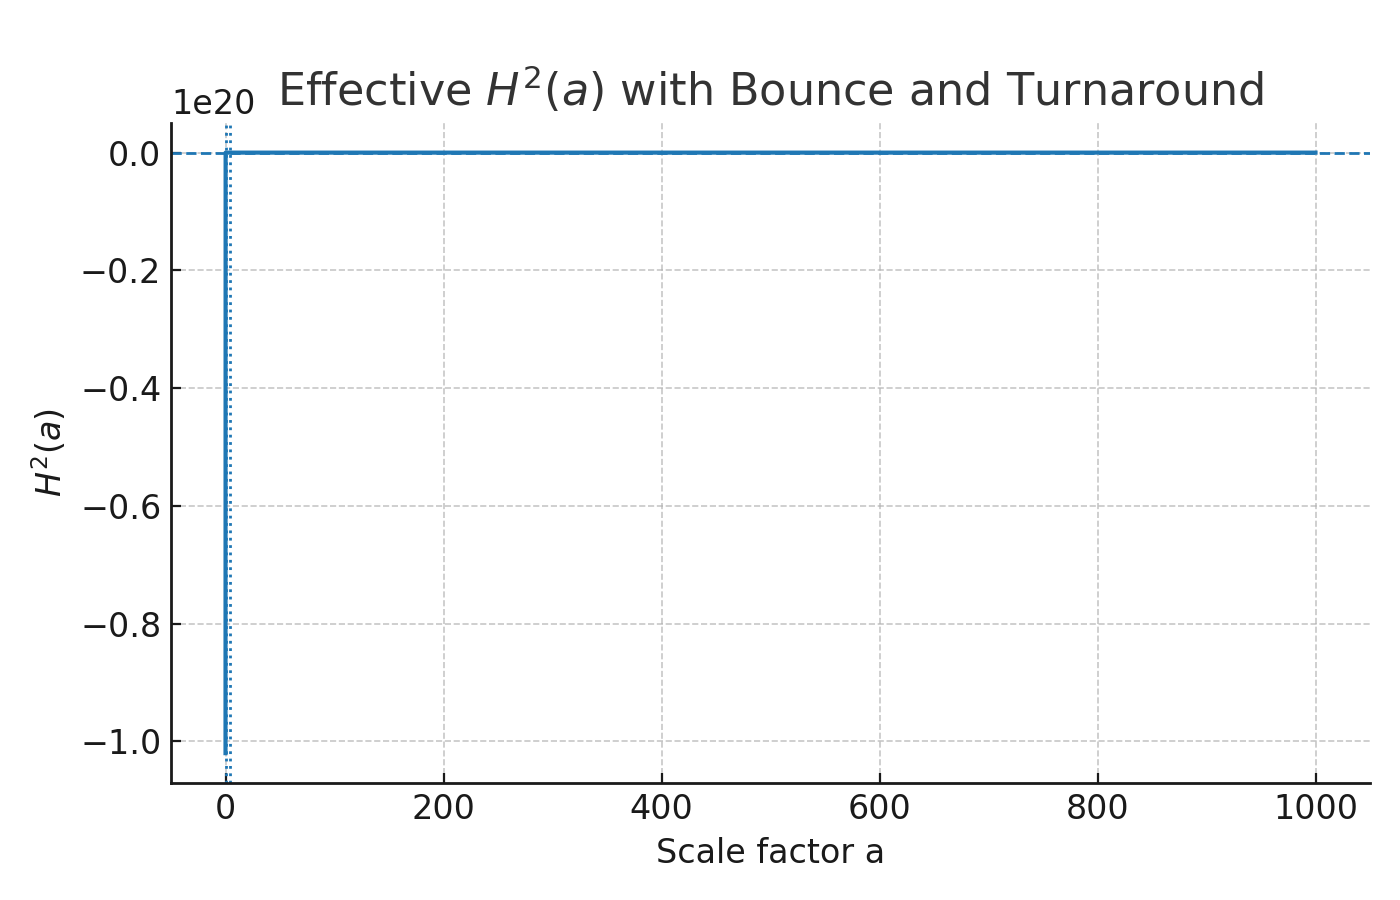
\includegraphics[width=0.7\linewidth]{figures/plot_H2_from_params.png}
\caption{Toy $H^2(a)$ exhibiting a small-$a$ bounce and a large-$a$ turnaround.}
\label{fig:h2a}
\end{figure}

\section{Discussion}
Compared to standard LQC \cite{Ashtekar2006}, this model retains the quantum bounce but introduces 
a built-in turnaround through closed time geometry. Unlike CCC \cite{Penrose2010}, which removes 
contraction via conformal mapping, this proposal preserves contraction and closes the cycle 
directly in time itself. The model also resonates with emergent-time perspectives such as the 
Hartle--Hawking wavefunction \cite{Hartle1983} and Rovelli's relational view of time \cite{Rovelli2017}. 

\paragraph{Bounce as a wavefunction.} In a Wheeler--DeWitt minisuperspace approximation, 
the universe wavefunction $\Psi(a)$ near $a_{\min}$ can be modeled as a Gaussian sharply 
peaked at $a_{\min}$, yielding a single-frame quantum state. Since $H=0$ at the bounce, 
extrinsic curvature vanishes and there is no relative time dilation between comoving observers.

\section{Conclusions and Next Steps}
We have presented a toy model embodying the idea of time as a closed controller loop. This framework 
unifies bounce and turnaround mechanisms in a geometric ansatz, offering a conceptual alternative to 
inflationary or purely conformal cyclic models. 

Future work should focus on deriving the effective dynamics from a fundamental theory of quantum gravity, 
and on observational predictions. For instance, perturbations can be evolved with
\begin{equation}
v_k''+(k^2-\tfrac{z''}{z})v_k=0,\qquad
\mu_k''+(k^2-\tfrac{a''}{a})\mu_k=0,
\end{equation}
to yield scalar/tensor spectra with potential signatures in the CMB and primordial gravitational waves. 
Entropy flow across cycles also warrants further study.

\section*{Acknowledgments}
The author thanks the open scientific community for providing freely accessible resources 
that make independent research possible. Foundational insights from Loop Quantum Cosmology, 
cyclic cosmology, and conformal cyclic cosmology by A.~Ashtekar, M.~Bojowald, P.~Steinhardt, 
N.~Turok, and R.~Penrose have provided inspiration for the framing of this note.

\begin{thebibliography}{9}

\bibitem{Ashtekar2006}
A.~Ashtekar, T.~Pawlowski, and P.~Singh,  
``Quantum nature of the big bang: Improved dynamics,''  
\emph{Phys. Rev. D}, vol. 74, p. 084003, 2006.  
doi:10.1103/PhysRevD.74.084003

\bibitem{Bojowald2001}
M.~Bojowald,  
``Absence of singularity in loop quantum cosmology,''  
\emph{Phys. Rev. Lett.}, vol. 86, p. 5227, 2001.  
doi:10.1103/PhysRevLett.86.5227

\bibitem{Steinhardt2002}
P.~J. Steinhardt and N.~Turok,  
``A cyclic model of the universe,''  
\emph{Science}, vol. 296, pp. 1436–1439, 2002.  
doi:10.1126/science.1070462

\bibitem{Penrose2010}
R.~Penrose,  
\emph{Cycles of Time: An Extraordinary New View of the Universe}.  
London: Bodley Head, 2010. ISBN: 978-0224080361

\bibitem{Hartle1983}
J.~B. Hartle and S.~W. Hawking,  
``Wave function of the Universe,''  
\emph{Phys. Rev. D}, vol. 28, pp. 2960–2975, 1983.  
doi:10.1103/PhysRevD.28.2960

\bibitem{Rovelli2017}
C.~Rovelli,  
\emph{Reality Is Not What It Seems: The Journey to Quantum Gravity}.  
Penguin Books, 2017. ISBN: 978-0735213920

\end{thebibliography}

\end{document}
